% Offizielle Beispieldatei für beamer-Vorlage aus tubslatex Version 0.3beta2
\documentclass[fleqn,11pt,aspectratio=43]{beamer}

\usepackage[ngerman]{babel}
\usepackage[utf8x]{inputenc}
\usepackage{graphicx}
\usepackage{minted}
\usetheme[%
  %nexus,%        Nexus Fonts benutzen
  %lnum,%         Versalziffern verwenden
  %cmyk,%<rgbprint>,          Auswahl des Farbmodells
  blue,%<orange/green/violet> Auswahl des Sekundärfarbklangs
  dark,%<light,medium>        Auswahl der Helligkeit
  %colorhead,%    Farbig hinterlegte Kopfleiste
  %colorfoot,%    Farbig hinterlegt Fußleiste auf Titelseite
  colorblocks,%   Blöcke Farbig hinterlegen
  %nopagenum,%    Keine Seitennumer in Fußzeile
  %nodate,%       Kein Datum in Fußleiste
  tocinheader,%   Inhaltsverzeichnis in Kopfleiste
  %tinytocinheader,% kleines Kopfleisten-Inhaltsverzeichnis
  %widetoc,%      breites Kopfleisten-Inhaltsverzeichnis
  %narrowtoc,%    schmales Kopfleisten-Inhaltsverzeichnis
  %nosubsectionsinheader,%  Keine subsections im Kopfleisten-Inhaltsverzeichnis
  %nologoinfoot,% Kein Logo im Fußbereich darstellen
  ]{tubs}

% Titelseite
\title{Dynamic Parallelism in CUDA}
\subtitle{The Mandelbrot Example}
\author{Marc Kassubeck}
% Titelgrafik, automatisch beschnitten, Weitere Optionen: <scaled/cropx/cropy>
% \titlegraphic[cropped]{\includegraphics{infozentrum.jpg}}
\titlegraphic[scaled]{
\includegraphics{titlepicture.jpg}}

% Logo, dass auf Titelseiten oben rechts und auf Inthaltsseiten unten rechts
% dargestellt wird. Es wird jeweils automatisch skliert
\logo{
\includegraphics{wire.jpeg}}
%\logo{Institut für Unkreativität\\und Schreibschwäche}

\begin{document}
\setminted{fontsize=\scriptsize, autogobble, breaklines, frame=single, tabsize=4}

\begin{frame}[plain]
\titlepage
\end{frame}

\begin{frame}[plain]
  \tableofcontents
\end{frame}


\section{The Mandelbrot Set}

\begin{frame}{Definition of the Mandelbrot Set}
	\begin{itemize}
		\item is a well known fractal
		\item consists of two parts
		\item definition of a series
	\end{itemize}	
	\begin{align*}
		z_0 &= c\\
		z_{n+1} &= z_n^2 + c
	\end{align*}
	\begin{itemize}
		\item defininition of the set in the complex plane
	\end{itemize}
	\begin{align*}
		M &= \{c \in \mathbb{C}: \exists R\ \forall n: \left| z_n \right| < R \}
	\end{align*}
	\begin{itemize}
		\item implementation won't check all $n$, but all $n$ up to a fixed number
	\end{itemize}
\end{frame}

\begin{frame}
	\begin{figure}
		
\includegraphics[height=0.9\textheight]{colored-mandelbrot-set.png}
		\caption{Visualisation of the Mandelbrot Set (black pixels)}
	\end{figure}
\end{frame}

\subsection{The Escape Time Algorithm}

\begin{frame}{The Escape Time Algorithm}
	\begin{itemize}
		\item one of the easiest algorithms for computing the Mandelbrot Set
		\item computes the \textit{dwell} for each pixel (point in the complex plane) according to the series definition
		\item for a fixed maximum number of iterations the series is computed and it is checked, if the value of \textit{dwell} 'escapes' outside a circle of radius 2
		\item this is correct, as the series will diverge, if one element lies outside this circle
		\item if the point 'escapes', the color value of the point will be the \textit{dwell}
		\item otherwise it will be black
	\end{itemize}
\end{frame}

\section{Computing the Mandelbrot Set in CUDA}

\begin{frame}[fragile]{The pixel dwell}
	This code block computes the dwell for a single pixel position:
	\begin{minted}{c++}
		#define MAX_DWELL 512
		// w, h --- width and hight of the image, in pixels
		// cmin, cmax --- coordinates of bottom-left and top-right image corners
		// x, y --- coordinates of the pixel
		__host__ __device__ int pixel_dwell(int w, int h, complex cmin, complex cmax, int x, int y) {
			complex dc = cmax - cmin;
			float fx = (float)x / w, fy = (float)y / h;
			complex c = cmin + complex(fx * dc.re, fy * dc.im);
			complex z = c; 
			int dwell = 0;
		
			while(dwell < MAX_DWELL && abs2(z) < 2 * 2) { 
				z = z * z + c;
				dwell++;
			}
			return dwell;
		}
	\end{minted}
\end{frame}

\begin{frame}[fragile]{Invoking the pixel-dwell-kernel}
	The easiest way to generate the Mandelbrot Set is to invoke the \textit{pixel\_dwell}-kernel for each pixel
	\begin{minted}{c++}
		__global__ void mandelbrot_k(int *dwells, int w, int h, complex cmin, complex cmax) {
			int x = threadIdx.x + blockDim.x * blockIdx.x;
			int y = threadIdx.y + blockDim.y * blockIdx.y;
			if(x < w && y < h)
				dwells[y * w + x] = pixel_dwell(w, h, cmin, cmax, x, y);
		}
	\end{minted}
	The kernel launch on the CPU
	\begin{minted}{c++}
	  int w = 4096, h = 4096;
	  dim3 bs(64, 4), grid(divup(w, bs.x), divup(h, bs.y));
	  mandelbrot_k <<<grid, bs>>>(d_dwells, w, h, complex(-1.5, 1), complex(0.5, 1));
	\end{minted}
\end{frame}

\section{Extending the Algorithm with Dynamic Parallelism}

\begin{frame}{Extending the Algorithm with Dynamic Parallelism}
	\begin{itemize}
		\item Extension relies on a mathematical fact
		\item The set is \textit{connected}
		\item Between any two parts of the set, there is a path, that lies wholly inside the set
		\item Thus, a region (of any shape) lies within the Mandelbrot Set, iff its border lies within the set
		\item More genrally, if the border of the region has a constant dwell, then every pixel in the region has the same dwell
		\item This saves computation time
	\end{itemize}
\end{frame}

\begin{frame}[fragile]{The Mariani-Silver Algorithm}
	The Mariani-Silver Algorithm combines the connectedness of the set with recursive subdivision of rectangular regions:
	\begin{minted}{c++}
	mariani_silver(rectangle) 
	  if (border(rectangle) has common dwell) 
	    fill rectangle with common dwell
	  else if (rectangle size < threshold)
	    per-pixel evaluation of the rectangle
	  else
	    for each sub_rectangle in subdivide(rectangle)
	      mariani_silver(sub_rectangle)
	\end{minted}
	In CUDA this will be implemented using one thread-block for each call of \textit{mariani\_silver}. This block then uses parallel reduction to determine the dwell of all border pixels and thread 0 then decides how to subdivide the rectangle
\end{frame}

\begin{frame}[fragile]{Mariani-Silver Algorithm using CUDA}
	\begin{minted}[fontsize=\tiny]{c++}
	__global__ void mandelbrot_block_k(int *dwells, int w, int h, complex cmin, complex cmax, int x0, int y0, int d, int depth) {
	
	x0 += d * blockIdx.x, y0 += d * blockIdx.y;
	int common_dwell = border_dwell(w, h, cmin, cmax, x0, y0, d);
	if (threadIdx.x == 0 && threadIdx.y == 0) {
		if (common_dwell != DIFF_DWELL) {
			// uniform dwell, just fill
			dim3 bs(BSX, BSY), grid(divup(d, BSX), divup(d, BSY)); 
			dwell_fill<<<grid, bs>>> (dwells, w, x0, y0, d, comm_dwell);
		} else if (depth + 1 > MAX_DEPTH && d / SUBDIV < MIN_SIZE) {
			// subdivide recursively
			dim3 bs(blockDim.x, blockDim.y), grid(SUBDIV, SUBDIV); 
			mandelbrot_block_k<<<grid, bs>>> (dwells, w, h, cmin, cmax, x0, y0, d / SUBDIV, depth+1);
		} else {
			// leaf, per-pixel kernel
			dim3 bs(BSX, BSY), grid(divup(d, BSX), divup(d, BSY)); 
			mandelbrot_pixel_k<<<grid, bs>>> (dwells, w, h, cmin, cmax, x0, y0, d);
		}
		cucheck_dev(cudaGetLastError());
		}
	}  // mandelbrot_block_k
	
	\end{minted}
\end{frame}

\begin{frame}[fragile]{Dwell Reduction}
	\begin{minted}{c++}
	/** binary operation for common dwell "reduction": MAX_DWELL + 1 = neutral
	element, -1 = dwells are different */
	#define NEUT_DWELL (MAX_DWELL + 1)
	#define DIFF_DWELL (-1)
	__device__ int same_dwell(int d1, int d2) {
		if (d1 == d2)
			return d1;
		else if (d1 == NEUT_DWELL || d2 == NEUT_DWELL)
			return min(d1, d2);
		else
			return DIFF_DWELL;
	}  // same_dwell
	\end{minted}
\end{frame}

\begin{frame}[fragile]{Dwell Reduction}
	\begin{minted}[fontsize=\tiny]{c++}
	__device__ int border_dwell (int w, int h, complex cmin, complex cmax, int x0, int y0, int d) {
	// check whether all boundary pixels have the same dwell
		int tid = threadIdx.y * blockDim.x + threadIdx.x;
		int bs = blockDim.x * blockDim.y;
		int comm_dwell = NEUT_DWELL;
		// for all boundary pixels, distributed across threads
		for (int r = tid; r < d; r += bs) {
			// for each boundary: b = 0 is east, then counter-clockwise
			for (int b = 0; b < 4; b++) {
				int x = b % 2 != 0 ? x0 + r : (b == 0 ? x0 + d - 1 : x0);
				int y = b % 2 == 0 ? y0 + r : (b == 1 ? y0 + d - 1 : y0);
				int dwell = pixel_dwell(w, h, cmin, cmax, x, y);
				comm_dwell = same_dwell(comm_dwell, dwell);
			}
		}  // for all boundary pixels
		// reduce across threads in the block
		__shared__ int ldwells[BSX * BSY];
		int nt = min(d, BSX * BSY);
		if (tid < nt)
			ldwells[tid] = comm_dwell;
		__syncthreads();
		for (; nt > 1; nt /= 2) {
			if (tid < nt / 2)
				ldwells[tid] = same_dwell(ldwells[tid], ldwells[tid + nt / 2]);
			__syncthreads();
		}
		return ldwells[0];
	}  // border_dwell
	\end{minted}
\end{frame}

\begin{frame}
	\begin{figure}
		
\includegraphics[height=0.9\textheight]{mariani-silver-subdivision.png}
		\caption{Recursive subdivision of the Mandelbrot Set}
	\end{figure}
\end{frame}

\subsection{Compiling the Algorithm for Dynamic Paralellism}

\begin{frame}{Compiling and Linking for Dynamic Parallelism}
	\begin{figure}
		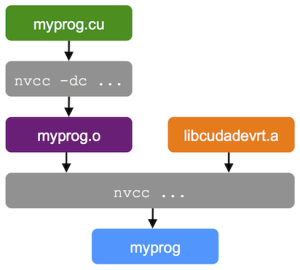
\includegraphics[width=0.33\textwidth]{dyn-compile-link.png}
		\caption{Two step compilation and linking for Dynamic Parallism}
	\end{figure}
	For creating a program using Dynamic Parallelism, the code must be built for Compute Capability 3.5 or higher and must be linked against \texttt{cudadevrt}
\end{frame}

\begin{frame}
	To compile into and object file, use the \texttt{-c}(\texttt{--compile}) option.\\
	To be able to link this object file later on, use \texttt{-rdc=true}(\texttt{--relocatable-device-code=true})\\
	\\
	Those two options can be shortened to \texttt{-dc}(\texttt{--device -c}):\\
	\texttt{nvcc -arch=sm\_35 -dc myprog.cu -o myprog.o}\\
	To link this object file with a library, use \texttt{-l} option of \texttt{nvcc}:\\
	\texttt{nvcc -arch=sm\_35 myprog.o -lcudadevrt -o myprog}\\
	\\
	One can also compile and link in a single step:\\
	\texttt{nvcc -arch=sm\_35 -rdc=true myprog.cu -lcudadevrt -o myprog.o}
\end{frame}

\end{document}
